% =====================================================================
% Rapport de projet — Finance Paiements
% Compilation : latexmk -pdf rapport.tex   (pdfLaTeX)
% =====================================================================
\documentclass[11pt,a4paper]{report}

% ---------------------------------------------------------------------
% Paramètres du document
% ---------------------------------------------------------------------
\newcommand{\Auteur}{LUMU BAMANA MANASSE}
\newcommand{\Titre}{Finance Paiements}
\newcommand{\SousTitre}{Portefeuille électronique et paiements numériques}
\newcommand{\Version}{1.1.0}
\newcommand{\DateDebut}{août 2026}
\newcommand{\DateMaj}{22 octobre 2026}
\newcommand{\Depot}{https://github.com/MediJr/finance-paiements}

% ---------------------------------------------------------------------
% Paquets
% ---------------------------------------------------------------------
\usepackage[utf8]{inputenc}
\usepackage[T1]{fontenc}
\usepackage[french]{babel}
\usepackage{lmodern}
\usepackage{microtype}
\usepackage[a4paper,margin=2.4cm,headheight=14pt]{geometry}
\usepackage[dvipsnames,table]{xcolor}
\usepackage{graphicx}
\usepackage{booktabs,tabularx,longtable,array,multirow}
\usepackage{enumitem}
\usepackage{caption}
\usepackage{float}
\usepackage{fancyhdr}
\usepackage{titlesec}
\usepackage{listings}
\usepackage{tikz}
\usetikzlibrary{positioning,arrows.meta,shapes.geometric,fit,calc}
\usepackage[most]{tcolorbox}
\usepackage{csquotes}
\usepackage[hidelinks]{hyperref}

\graphicspath{{../captures/}}

% ---------------------------------------------------------------------
% Couleurs et mise en forme
% ---------------------------------------------------------------------
\definecolor{primaire}{HTML}{0F6E5C}
\definecolor{primaireclair}{HTML}{E7F3F0}
\definecolor{encre}{HTML}{1B2A33}
\definecolor{gris}{HTML}{5B6770}
\definecolor{rouge}{HTML}{B42318}
\definecolor{orange}{HTML}{B54708}
\definecolor{jaune}{HTML}{A16207}
\definecolor{bleu}{HTML}{175CD3}

\hypersetup{
  colorlinks=true, linkcolor=primaire, urlcolor=primaire, citecolor=primaire,
  pdftitle={\Titre{} — Rapport de projet}, pdfauthor={\Auteur},
}

\setlength{\parindent}{0pt}
\setlength{\parskip}{0.55em}
\renewcommand{\arraystretch}{1.25}
\setlist{itemsep=0.15em, topsep=0.3em}
\captionsetup{font=small, labelfont={bf,color=primaire}}

\titleformat{\chapter}[display]
  {\normalfont\bfseries\color{encre}}
  {\color{primaire}\large\MakeUppercase{\chaptertitlename}~\thechapter}
  {0.4em}{\Huge}[{\color{primaire}\titlerule[1.2pt]}]
\titlespacing*{\chapter}{0pt}{-10pt}{22pt}
\titleformat{\section}{\normalfont\Large\bfseries\color{encre}}{\color{primaire}\thesection}{0.8em}{}
\titleformat{\subsection}{\normalfont\large\bfseries\color{encre}}{\color{primaire}\thesubsection}{0.8em}{}

\pagestyle{fancy}
\fancyhf{}
\fancyhead[L]{\small\color{gris}\Titre{} — Rapport de projet}
\fancyhead[R]{\small\color{gris}\nouppercase{\leftmark}}
\fancyfoot[L]{\small\color{gris}\Auteur}
\fancyfoot[R]{\small\color{gris}\thepage}
\renewcommand{\headrulewidth}{0.4pt}
\fancypagestyle{plain}{\fancyhf{}\fancyfoot[R]{\small\color{gris}\thepage}\renewcommand{\headrulewidth}{0pt}}

% Encadrés
\newtcolorbox{encadre}[1][]{colback=primaireclair, colframe=primaire, boxrule=0.6pt,
  arc=2pt, left=8pt, right=8pt, top=6pt, bottom=6pt, fonttitle=\bfseries, #1}

% En-tête de tableau
\newcommand{\entete}{\rowcolor{primaire}}
\newcommand{\tete}[1]{\textcolor{white}{\textbf{#1}}}
\newcolumntype{Y}{>{\raggedright\arraybackslash}X}
\newcolumntype{C}[1]{>{\centering\arraybackslash}p{#1}}

% Code
\lstdefinestyle{python}{
  language=Python, basicstyle=\ttfamily\small, keywordstyle=\color{primaire}\bfseries,
  commentstyle=\color{gris}\itshape, stringstyle=\color{orange},
  backgroundcolor=\color{primaireclair!50}, frame=single, rulecolor=\color{primaire!40},
  breaklines=true, columns=fullflexible, showstringspaces=false,
  numbers=left, numberstyle=\tiny\color{gris}, xleftmargin=1.8em, framexleftmargin=1.5em,
  literate={é}{{\'e}}1 {è}{{\`e}}1 {à}{{\`a}}1 {ê}{{\^e}}1 {ç}{{\c{c}}}1 {É}{{\'E}}1
           {ù}{{\`u}}1 {î}{{\^i}}1 {ô}{{\^o}}1 {•}{{\textbullet}}1 {→}{{$\rightarrow$}}1,
}
\lstset{style=python}

\newcommand{\code}[1]{\texttt{\small #1}}
\newcommand{\gravite}[2]{\textcolor{#1}{\textbf{#2}}}

% =====================================================================
\begin{document}

% ---------------------------------------------------------------------
% Page de garde
% ---------------------------------------------------------------------
\begin{titlepage}
\newgeometry{margin=0cm}
\begin{tikzpicture}[remember picture, overlay]
  \fill[primaire] (current page.north west) rectangle ([yshift=-9.5cm]current page.north east);
  \fill[primaire!80!black] ([yshift=-9.5cm]current page.north west) rectangle ([yshift=-9.8cm]current page.north east);
  \node[anchor=north west, text=white, align=left] at ([xshift=2.4cm,yshift=-2.6cm]current page.north west)
    {\fontsize{12}{14}\selectfont\bfseries RAPPORT DE PROJET — DÉVELOPPEMENT LOGICIEL};
  \node[anchor=north west, text=white, align=left] at ([xshift=2.4cm,yshift=-3.7cm]current page.north west)
    {\fontsize{38}{44}\selectfont\bfseries \Titre};
  \node[anchor=north west, text=white!90!primaire, align=left] at ([xshift=2.4cm,yshift=-5.6cm]current page.north west)
    {\fontsize{20}{24}\selectfont \SousTitre};
  \node[anchor=north west, text=white!85!primaire, align=left, text width=16cm] at ([xshift=2.4cm,yshift=-7.0cm]current page.north west)
    {\large Analyse, conception, réalisation, tests, audit de sécurité et déploiement\\ d'une plateforme de portefeuille électronique};
\end{tikzpicture}

\vspace*{11.5cm}
\hspace{2.4cm}%
\begin{minipage}{16.2cm}
  {\color{gris}\large Réalisé par}\\[0.3em]
  {\fontsize{24}{28}\selectfont\bfseries\color{encre} \Auteur}

  \vspace{1.6cm}
  \renewcommand{\arraystretch}{1.6}
  \begin{tabular}{@{}>{\color{gris}}l@{\hspace{1.2cm}}>{\color{encre}\bfseries}l@{}}
    Début du projet        & \DateDebut \\
    Dernière mise à jour   & \DateMaj \\
    Version                & \Version \\
    Modèle de cycle de vie & Prototypage évolutif \\
    Méthode                & Agile — Scrum (5 prototypes, 12 sprints) \\
    Technologies           & Python 3.12 · Django 6 · Django REST Framework \\
                           & PostgreSQL 16 · Docker · GitHub Actions \\
    Code source            & \href{\Depot}{\nolinkurl{github.com/MediJr/finance-paiements}} \\
  \end{tabular}
\end{minipage}

\vfill
\begin{tikzpicture}[remember picture, overlay]
  \fill[primaireclair] (current page.south west) rectangle ([yshift=2.2cm]current page.south east);
  \node[anchor=west, text=gris] at ([xshift=2.4cm,yshift=1.1cm]current page.south west)
    {\small 169 tests automatisés \quad·\quad 86\,\% de couverture \quad·\quad 11 défauts corrigés lors de l'audit \quad·\quad Licence MIT};
\end{tikzpicture}
\restoregeometry
\end{titlepage}

% ---------------------------------------------------------------------
% Résumé
% ---------------------------------------------------------------------
\pagenumbering{roman}
\chapter*{Résumé}
\addcontentsline{toc}{chapter}{Résumé}
\markboth{Résumé}{}

\textbf{Finance Paiements} est une plateforme de \textbf{portefeuille électronique}.
Chaque client dispose d'un portefeuille en euros qu'il alimente par carte bancaire,
avec lequel il vire de l'argent à ses proches, paie des commerçants et reçoit des
remboursements. Le personnel supervise l'activité, fixe les plafonds, peut suspendre
les opérations et consulte journaux, statistiques et exports. Les fonctions sont
accessibles par une interface web et par une API REST.

Le logiciel a été développé selon le \textbf{modèle par prototypage évolutif} :
cinq prototypes fonctionnels successifs, chacun enrichissant le précédent. À
l'intérieur de chaque prototype, le travail a été organisé selon la méthode
\textbf{agile Scrum}, en douze sprints (0 à 11), l'auteur tenant lui-même le rôle du
client lors de l'évaluation de chaque prototype.

Ce rapport retrace toutes les phases du cycle de vie du développement logiciel :
l'\textbf{analyse des besoins} (15 exigences fonctionnelles, 13 exigences non
fonctionnelles, 20 récits utilisateurs), la \textbf{conception} (architecture en
couches, module unique de mouvements de fonds, modèle de données), la
\textbf{réalisation} sprint par sprint, les \textbf{tests} (169 tests automatisés,
86\,\% de couverture, matrice de traçabilité), l'\textbf{audit de sécurité} mené par
l'auteur sur son propre code (11 défauts identifiés et corrigés), le
\textbf{déploiement} et la \textbf{maintenance}.

\begin{encadre}[title=Chiffres clés]
\begin{tabularx}{\linewidth}{@{}YYYY@{}}
\textbf{\Large 11} modèles de données & \textbf{\Large 31} routes d'API REST & \textbf{\Large 35} pages web & \textbf{\Large 169} tests automatisés \\
\textbf{\Large 86\,\%} de couverture & \textbf{\Large 12} sprints & \textbf{\Large 11} défauts corrigés & \textbf{\Large 0} alerte de configuration \\
\end{tabularx}
\end{encadre}

\tableofcontents
\listoffigures
\listoftables

\cleardoublepage
\pagenumbering{arabic}

% =====================================================================
\chapter{Présentation du logiciel}
% =====================================================================

\section{Contexte}

Les applications de paiement entre particuliers et les néobanques ont popularisé le
portefeuille électronique : un solde en ligne que l'on approvisionne une fois, puis que
l'on utilise pour envoyer ou recevoir de l'argent instantanément. Un établissement
fictif souhaite proposer ce service à ses clients, avec un haut niveau d'exigence sur
l'intégrité des fonds, la confidentialité et la traçabilité.

\section{À quoi sert le logiciel}

\begin{description}[leftmargin=0pt, labelsep=0.6em]
  \item[Pour le client] ouvrir un compte, alimenter son portefeuille par carte, gérer
  ses bénéficiaires, effectuer des virements et des paiements, rembourser un paiement
  reçu, consulter son historique.
  \item[Pour l'établissement] superviser utilisateurs, portefeuilles et opérations,
  activer ou désactiver un compte, fixer les plafonds (par opération, journalier,
  d'alimentation), suspendre les opérations (mode maintenance).
  \item[Pour la direction] suivre l'activité par un tableau de bord, des statistiques
  et des rapports ; exporter les données en CSV ou JSON.
  \item[Pour l'audit] disposer d'un journal immuable des événements
  sensibles (connexions, alimentations, virements, actions d'administration).
\end{description}

\section{Acteurs}

\begin{table}[H]
\centering
\caption{Acteurs du système}
\begin{tabularx}{\linewidth}{@{}lY@{}}
\toprule
\entete \tete{Acteur} & \tete{Rôle} \\
\midrule
Visiteur & Crée un compte et se connecte. \\
Client & Possède un portefeuille ; alimente, vire, paie, rembourse, consulte. \\
Administrateur & Membre du personnel ; supervise, paramètre, active ou désactive des comptes, consulte journaux et exports. \\
\bottomrule
\end{tabularx}
\end{table}

\section{Aperçu}

\begin{figure}[H]
\centering
\begin{minipage}{0.49\linewidth}\centering
  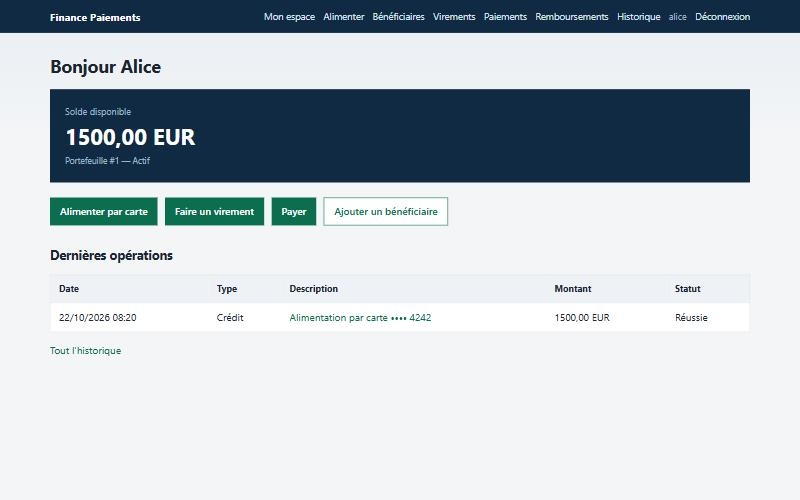
\includegraphics[width=\linewidth]{01-espace-client.jpg}\\[-0.2em]
  {\small (a) Espace client}
\end{minipage}\hfill
\begin{minipage}{0.49\linewidth}\centering
  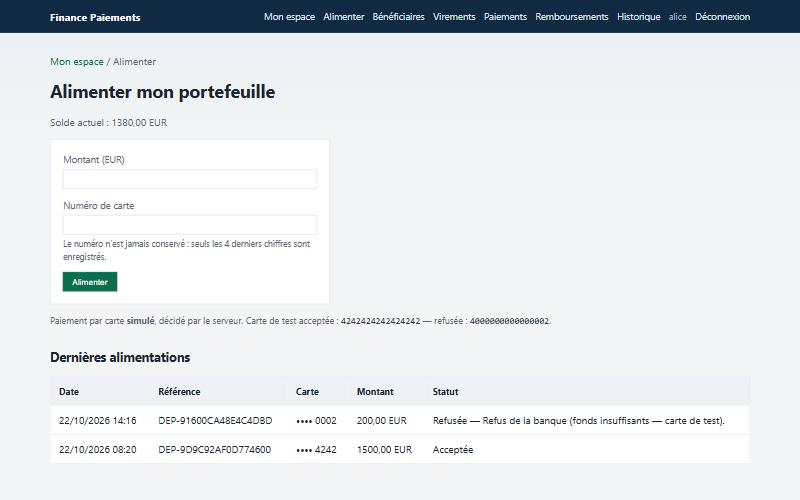
\includegraphics[width=\linewidth]{02-alimentation.jpg}\\[-0.2em]
  {\small (b) Alimentation par carte}
\end{minipage}
\caption{Interface client : solde, actions rapides et alimentation}
\end{figure}

\section{Périmètre}

Le traitement de la carte bancaire est \textbf{simulé} : une passerelle côté serveur
reproduit le comportement d'un prestataire (validation du numéro, autorisation, refus,
masquage). Sont hors périmètre : un prestataire de paiement réel, les virements vers un
compte bancaire externe, le multi-devise avec conversion, la vérification d'identité
(KYC) et les notifications par e-mail ou SMS.

% =====================================================================
\chapter{Démarche : modèle de cycle de vie et méthode}
% =====================================================================

\section{Modèle : le prototypage évolutif}

Le projet suit le \textbf{modèle par prototypage évolutif}. Le logiciel est construit
sous forme de prototypes successifs ; chaque prototype est \emph{fonctionnel},
\emph{testé} et \emph{utilisable}. Il n'est pas jeté après évaluation mais
\textbf{enrichi} par le suivant, jusqu'au produit final.

\begin{figure}[H]
\centering
\begin{tikzpicture}[
  node distance=0.45cm and 0.5cm,
  proto/.style={rectangle, rounded corners=3pt, draw=primaire, fill=primaireclair, thick,
                minimum width=2.15cm, minimum height=1.25cm, align=center, font=\small},
  eval/.style={diamond, aspect=1.6, draw=gris, fill=white, inner sep=1pt, font=\scriptsize, align=center},
  fleche/.style={-{Stealth[length=2.2mm]}, thick, color=encre},
]
  \node[proto, fill=white, draw=gris] (b) {Besoins\\initiaux};
  \node[proto, right=of b] (p1) {\textbf{P1}\\Fondation\\{\scriptsize S0--S2}};
  \node[proto, right=of p1] (p2) {\textbf{P2}\\Opérations\\{\scriptsize S3--S5}};
  \node[proto, right=of p2] (p3) {\textbf{P3}\\Admin. et\\sécurité {\scriptsize S6--S8}};
  \node[proto, right=of p3] (p4) {\textbf{P4}\\Exploitation\\{\scriptsize S9--S10}};
  \node[proto, right=of p4, fill=primaire, text=white] (p5) {\textbf{P5}\\Durcissement\\{\scriptsize S11}};
  \foreach \a/\c in {b/p1, p1/p2, p2/p3, p3/p4, p4/p5} \draw[fleche] (\a) -- (\c);
  \foreach \a/\c/\k in {p1/p2/1, p2/p3/2, p3/p4/3, p4/p5/4} {
    \coordinate (m\k) at ($(\a.south)!0.5!(\c.south) + (0,-1.15)$);
    \node[eval] (e\k) at (m\k) {évaluation};
    \draw[fleche, dashed, color=gris] (\a.south) |- (e\k.west);
    \draw[fleche, dashed, color=gris] (e\k.east) -| (\c.south);
  }
  \node[font=\scriptsize, text=rouge, below=0.05cm of e4] {audit de sécurité};
\end{tikzpicture}
\caption{Prototypage évolutif : cinq prototypes successifs, chacun évalué avant le suivant}
\end{figure}

\begin{table}[H]
\centering
\caption{Justification du choix du modèle}
\begin{tabularx}{\linewidth}{@{}p{4.6cm}Y@{}}
\toprule
\entete \tete{Critère} & \tete{Justification} \\
\midrule
Besoins qui se précisent en cours de route & Un portefeuille électronique se comprend en le manipulant : l'impossibilité d'approvisionner un portefeuille n'est apparue qu'en jouant le parcours complet du prototype 4. \\
Risques maîtrisés tôt & Le cœur sensible --- les mouvements de fonds atomiques --- est construit et testé dès le prototype 2, avant toute interface d'administration. \\
Sécurité par couches & Le prototype 3 est consacré à la \emph{Security by Design}, le prototype 5 à l'audit et au durcissement. \\
Développeur unique & Pas de lourdeur documentaire initiale : la documentation grandit avec le produit. \\
\bottomrule
\end{tabularx}
\end{table}

\section{Méthode : Agile Scrum adapté}

À l'intérieur de chaque prototype, le travail est découpé en \textbf{sprints} courts
selon la méthode \textbf{Scrum}. Le projet étant mené par une seule personne, les rôles
et les cérémonies ont été adaptés : l'auteur est à la fois Product Owner, équipe de
développement et client lors des évaluations.

\begin{table}[H]
\centering
\caption{Mise en œuvre de Scrum}
\begin{tabularx}{\linewidth}{@{}p{4.2cm}Y@{}}
\toprule
\entete \tete{Élément Scrum} & \tete{Mise en œuvre dans le projet} \\
\midrule
Product Owner & L'auteur définit et priorise le backlog (méthode MoSCoW). \\
Équipe de développement & L'auteur. \\
Client & L'auteur, dans le rôle d'utilisateur final : chaque prototype est évalué en le manipulant comme client puis comme administrateur. \\
Product backlog & 20 récits utilisateurs reliés aux exigences (\code{docs/backlog.md}). \\
Sprint planning & Objectif de sprint et récits sélectionnés, en tête de chaque rapport de sprint. \\
Incrément & Code, migrations, tests et documentation livrés ensemble. \\
Sprint review & Démonstration du parcours et validation de l'objectif. \\
Rétrospective & Section « Limites / suite » des rapports de sprint, reprise au sprint suivant. \\
\bottomrule
\end{tabularx}
\end{table}

\subsection*{Definition of Done}

Un récit utilisateur est considéré comme \textbf{terminé} lorsque :
\begin{enumerate}
  \item le code est écrit dans la couche adaptée (service métier, puis vue ou API) ;
  \item toute modification de solde passe par le module de mouvements de fonds ;
  \item les migrations sont générées et \code{makemigrations --check} ne détecte rien ;
  \item des tests automatisés couvrent le cas nominal \emph{et} les cas d'erreur ;
  \item la suite complète de tests passe ;
  \item les actions sensibles sont journalisées (à partir du sprint 9) ;
  \item la documentation du module et le rapport de sprint sont à jour.
\end{enumerate}

\section{Phases du cycle de vie et livrables}

\begin{table}[H]
\centering
\caption{Phases du cycle de vie et livrables correspondants dans le dépôt}
\begin{tabularx}{\linewidth}{@{}p{3.4cm}Yp{4.6cm}@{}}
\toprule
\entete \tete{Phase} & \tete{Contenu} & \tete{Livrables} \\
\midrule
1. Analyse des besoins & Contexte, acteurs, exigences, récits utilisateurs & \code{cahier-des-charges.md}, \code{backlog.md} \\
2. Conception & Architecture, modèle de données, flux de fonds & \code{architecture.md} \\
3. Réalisation & Développement incrémental par sprints & Code, \code{livrables/Sprint-XX} \\
4. Tests & Unitaires, intégration, sécurité, CI & \code{tests/}, \code{tests.md}, CI \\
5. Audit et validation & Audit technique et de sécurité, remédiation & \code{securite.md}, \code{livrables/Audit} \\
6. Déploiement & Docker, production & \code{docker/}, \code{installation.md} \\
7. Maintenance & Historique, versions, évolutions & \code{CHANGELOG.md}, \code{versions.md} \\
\bottomrule
\end{tabularx}
\end{table}

% =====================================================================
\chapter{Analyse des besoins}
% =====================================================================

L'analyse des besoins formalise ce que le logiciel doit faire (\emph{exigences
fonctionnelles}) et les qualités qu'il doit présenter (\emph{exigences non
fonctionnelles}). Chaque exigence est numérotée afin d'être reliée au code puis aux
tests qui la vérifient (section~\ref{sec:tracabilite}). La priorité suit la méthode
\textbf{MoSCoW} : \textbf{M} (\emph{Must}, indispensable), \textbf{S} (\emph{Should},
importante), \textbf{C} (\emph{Could}, souhaitable).

\section{Exigences fonctionnelles}

\begin{longtable}{@{}p{1.3cm}p{10.4cm}C{1cm}C{1.5cm}@{}}
\caption{Exigences fonctionnelles}\\
\toprule
\entete \tete{ID} & \tete{Exigence} & \tete{Prio.} & \tete{Sprint} \\
\midrule
\endfirsthead
\toprule
\entete \tete{ID} & \tete{Exigence} & \tete{Prio.} & \tete{Sprint} \\
\midrule
\endhead
\multicolumn{4}{@{}l}{\textit{\color{primaire} Comptes et portefeuilles}} \\
EF-01 & Un visiteur crée un compte ; un portefeuille en euros à solde nul est ouvert automatiquement. & M & 1, 11 \\
EF-02 & Un client se connecte et se déconnecte depuis un espace dédié, distinct du site d'administration. & M & 11 \\
EF-03 & Un client consulte son solde, son profil et ses dernières opérations. & M & 1, 11 \\
EF-04 & Un client alimente son portefeuille par carte ; la passerelle accepte ou refuse. & M & 11 \\
\multicolumn{4}{@{}l}{\textit{\color{primaire} Opérations}} \\
EF-05 & Chaque opération est inscrite dans un historique consultable et filtrable. & M & 2 \\
EF-06 & Un client gère ses bénéficiaires (ajout par adresse e-mail, alias, désactivation). & M & 3, 11 \\
EF-07 & Un client vire de l'argent à un bénéficiaire actif ; débit et crédit sont atomiques. & M & 4 \\
EF-08 & Un client paie un bénéficiaire, qui peut le rembourser totalement ou partiellement. & M & 5 \\
EF-09 & Une demande envoyée deux fois (double clic, réseau) n'est exécutée qu'une fois. & M & 11 \\
\multicolumn{4}{@{}l}{\textit{\color{primaire} Administration et pilotage}} \\
EF-10 & Supervision des utilisateurs, portefeuilles et opérations ; activation et désactivation des comptes. & M & 6 \\
EF-11 & Paramètres : plafonds par opération, journalier et d'alimentation, devise, durée de session, mode maintenance. & M & 6, 7, 11 \\
EF-12 & Les actions d'administration sont journalisées. & M & 7 \\
EF-13 & Tableau de bord, statistiques et rapports filtrables. & S & 8 \\
EF-14 & Journal d'événements centralisé et consultable. & S & 9 \\
EF-15 & Export CSV / JSON de 8 jeux de données. & C & 10 \\
\bottomrule
\end{longtable}

\section{Exigences non fonctionnelles}

\begin{longtable}{@{}p{1.4cm}p{2.5cm}p{6.1cm}p{4.1cm}@{}}
\caption{Exigences non fonctionnelles}\\
\toprule
\entete \tete{ID} & \tete{Catégorie} & \tete{Exigence} & \tete{Mise en œuvre} \\
\midrule
\endfirsthead
\toprule
\entete \tete{ID} & \tete{Catégorie} & \tete{Exigence} & \tete{Mise en œuvre} \\
\midrule
\endhead
ENF-01 & Sécurité & Mots de passe hachés et validés ; message d'échec identique que le compte existe ou non. & Validateurs Django, PBKDF2 \\
ENF-02 & Sécurité & Un client n'accède qu'à ses données ; administration réservée au personnel. & Filtrage dans les services \\
ENF-03 & Sécurité & Aucun annuaire de clients exposé. & Ajout par e-mail exact \\
ENF-04 & Sécurité & Blocage après 5 échecs de connexion (compte) ou 20 (IP). & \code{auth\_service} + cache \\
ENF-05 & Sécurité & CSRF, XSS, clickjacking, redirections ouvertes, injection CSV. & Middleware, \code{commun/} \\
ENF-06 & Sécurité & Aucune donnée de carte complète conservée. & \code{carte\_masquee} \\
ENF-07 & Intégrité & Ni solde négatif ni double débit. & Transactions, verrous, idempotence \\
ENF-08 & Intégrité & Montants décimaux à 2 décimales, sans arrondi silencieux. & \code{parse\_montant} \\
ENF-09 & Conformité & Plafond par opération et plafond journalier cumulé. & \code{securite\_service} \\
ENF-10 & Traçabilité & Événements immuables pour toute action sensible. & \code{journal\_service} \\
ENF-11 & Qualité & Couverture $\geq 80$\,\%, tests à chaque push. & pytest-cov, GitHub Actions \\
ENF-12 & Déploiement & Démarrage refusé sans clé secrète ; HTTPS en production. & \code{settings/production.py} \\
ENF-13 & Maintenabilité & Un seul module modifie les soldes ; logique dans les services. & \code{mouvement\_service} \\
\bottomrule
\end{longtable}

\section{Récits utilisateurs}

Les exigences ont été traduites en \textbf{20 récits utilisateurs} au format
« En tant que\dots{} je veux\dots{} afin de\dots{} ». Quelques exemples :

\begin{table}[H]
\centering
\caption{Extrait du product backlog}
\begin{tabularx}{\linewidth}{@{}p{1.2cm}Yp{2.2cm}C{1.2cm}@{}}
\toprule
\entete \tete{ID} & \tete{Récit utilisateur} & \tete{Exigence} & \tete{Sprint} \\
\midrule
US-05 & En tant que client, je veux virer de l'argent à un bénéficiaire, sans risque de débit sans crédit. & EF-07, ENF-07 & 4 \\
US-08 & En tant qu'administrateur, je veux fixer des plafonds et suspendre les opérations en cas d'incident. & EF-11 & 6, 7 \\
US-09 & En tant que client, je veux être certain qu'aucun autre client ne voit mes données. & ENF-02 & 7 \\
US-15 & En tant que client, je veux alimenter mon portefeuille par carte afin de pouvoir l'utiliser. & EF-04 & 11 \\
US-16 & En tant que client, je veux qu'un double clic ne me débite jamais deux fois. & EF-09 & 11 \\
US-17 & En tant que client, je veux que personne ne puisse obtenir la liste des clients. & ENF-03 & 11 \\
\bottomrule
\end{tabularx}
\end{table}

\section{Contraintes}

\begin{itemize}
  \item Technologies : Python 3.12, Django 6, Django REST Framework, PostgreSQL 16.
  \item Projet mené par une seule personne, qui tient aussi le rôle de Product Owner.
  \item Données de démonstration uniquement ; aucune transaction bancaire réelle.
\end{itemize}

% =====================================================================
\chapter{Conception}
% =====================================================================

\section{Architecture en couches}

L'application est un monolithe Django \textbf{modulaire}. L'interface web et l'API REST
partagent une même \textbf{couche de services métier}. Un module unique,
\code{mouvement\_service}, est autorisé à débiter et à créditer les portefeuilles.

\begin{figure}[H]
\centering
\begin{tikzpicture}[
  couche/.style={rectangle, rounded corners=3pt, draw=primaire, thick, fill=primaireclair,
                 minimum height=1cm, align=center, font=\small, text width=3.6cm},
  ext/.style={rectangle, rounded corners=3pt, draw=gris, fill=white, minimum height=0.9cm,
              align=center, font=\small, text width=3.2cm},
  fleche/.style={-{Stealth[length=2mm]}, thick, color=encre},
  etiquette/.style={font=\scriptsize\bfseries, text=gris, anchor=east},
]
  \node[ext] (nav) at (0,0) {Navigateur};
  \node[ext] (cli) at (5,0) {Client API / mobile};
  \node[couche] (web) at (0,-1.8) {Vues web\\{\scriptsize gabarits Django}};
  \node[couche] (api) at (5,-1.8) {API REST\\{\scriptsize Django REST Framework}};
  \node[couche, text width=9cm, fill=primaire, text=white] (svc) at (2.5,-3.6) {\textbf{Services métier}\\{\scriptsize règles, plafonds, maintenance, cloisonnement, idempotence}};
  \node[couche, text width=2.6cm] (gw) at (-1.2,-5.4) {Passerelle\\carte simulée};
  \node[couche, text width=3.6cm, fill=primaire!25] (mvt) at (2.5,-5.4) {\textbf{\small mouvement\_service}\\{\scriptsize seul débit / crédit}};
  \node[couche, text width=2.6cm] (obs) at (6.2,-5.4) {Journal\\d'événements};
  \node[cylinder, shape border rotate=90, aspect=0.25, draw=primaire, thick, fill=white,
        minimum height=1.2cm, minimum width=2.6cm, font=\small] (db) at (2.5,-7.2) {PostgreSQL 16};
  \draw[fleche] (nav) -- (web);
  \draw[fleche] (cli) -- (api);
  \draw[fleche] (web) -- (svc.north -| web);
  \draw[fleche] (api) -- (svc.north -| api);
  \draw[fleche] (svc.south -| gw) -- (gw);
  \draw[fleche] (svc) -- (mvt);
  \draw[fleche] (svc.south -| obs) -- (obs);
  \draw[fleche] (mvt) -- (db);
  \draw[fleche] (obs.south) |- (db.east);
  \node[etiquette] at (-2.4,-1.8) {PRÉSENTATION};
  \node[etiquette] at (-2.4,-3.6) {MÉTIER};
  \node[etiquette] at (-2.4,-7.2) {DONNÉES};
\end{tikzpicture}
\caption{Architecture en couches}
\end{figure}

\begin{table}[H]
\centering
\caption{Modules (applications Django)}
\begin{tabularx}{\linewidth}{@{}p{3.2cm}Y@{}}
\toprule
\entete \tete{Module} & \tete{Rôle} \\
\midrule
\code{accounts} & Utilisateurs métier, inscription, connexion protégée, espace client \\
\code{wallets} & Portefeuilles, mouvements de fonds, alimentation par carte \\
\code{historique} & Journal des opérations de chaque portefeuille \\
\code{beneficiaires} & Destinataires autorisés (ajout par e-mail) \\
\code{virements} & Virements entre portefeuilles \\
\code{paiements} & Paiements et remboursements \\
\code{administration} & Paramètres, supervision, sécurité, pilotage, exports \\
\code{observabilite} & Journal d'événements immuable, erreurs HTTP 500 \\
\code{api} & Routes REST (client et administration) \\
\code{commun} & Adresse IP fiable, redirections sûres, clé d'idempotence \\
\bottomrule
\end{tabularx}
\end{table}

\section{Modèle de données}

\begin{figure}[H]
\centering
\begin{tikzpicture}[
  ent/.style={rectangle, draw=primaire, thick, fill=primaireclair, rounded corners=2pt,
              minimum width=2.7cm, minimum height=0.8cm, font=\small\bfseries},
  rel/.style={thick, color=gris},
  card/.style={font=\scriptsize, text=encre, fill=white, inner sep=1pt},
]
  \node[ent] (user) at (0,0) {User (Django)};
  \node[ent] (util) at (4,0) {Utilisateur};
  \node[ent] (benef) at (8.4,0) {Bénéficiaire};
  \node[ent] (wallet) at (4,-2.2) {Wallet};
  \node[ent] (alim) at (0,-2.2) {Alimentation};
  \node[ent] (vir) at (8.4,-2.2) {Virement};
  \node[ent] (hist) at (0,-4.4) {HistoriqueOpération};
  \node[ent] (pay) at (4,-4.4) {Paiement};
  \node[ent] (remb) at (8.4,-4.4) {Remboursement};
  \node[ent] (ev) at (0,1.9) {Événement};
  \node[ent] (param) at (8.4,1.9) {ParamètresApplication};

  \draw[rel] (user) -- node[card]{1--1} (util);
  \draw[rel] (util) -- node[card]{1--n} (benef);
  \draw[rel] (util) -- node[card]{1--1} (wallet);
  \draw[rel] (wallet) -- node[card]{1--n} (alim);
  \draw[rel] (wallet) -- node[card, align=center]{émet /\\reçoit} (vir);
  \draw[rel] (wallet) -- node[card, align=center]{paie /\\encaisse} (pay);
  \draw[rel] (pay) -- node[card]{1--n} (remb);
  \draw[rel] (wallet) -- node[card]{1--n} (hist);
  \draw[rel] (user) -- node[card]{1--n} (ev);
\end{tikzpicture}
\caption{Principales entités du modèle de données (11 modèles)}
\end{figure}

\paragraph{Choix de conception notables.}
\begin{itemize}
  \item \textbf{Solde jamais négatif} : le solde est contrôlé \emph{après} le
  verrouillage des deux portefeuilles, dans la même transaction que l'écriture.
  \item \textbf{Verrous dans un ordre stable} (identifiants triés) : deux virements
  croisés ne peuvent pas s'interbloquer.
  \item \textbf{Idempotence} : \code{Virement}, \code{Paiement} et \code{Alimentation}
  portent une clé unique par portefeuille émetteur, garantie par une contrainte en base.
  \item \textbf{Historique double} : chaque transfert écrit une ligne de sortie chez
  l'émetteur et une ligne d'entrée chez le destinataire.
  \item \textbf{Paramètres singleton} : une seule ligne de paramètres globaux, éditable
  par l'administration et journalisée.
\end{itemize}

\section{Flux d'un virement}

\begin{figure}[H]
\centering
\begin{tikzpicture}[xscale=1.17,
  acteur/.style={rectangle, draw=primaire, thick, fill=primaireclair, rounded corners=2pt,
                 minimum width=2.4cm, minimum height=0.75cm, font=\scriptsize\bfseries},
  msg/.style={-{Stealth[length=1.8mm]}, thick, color=encre},
  ret/.style={-{Stealth[length=1.8mm]}, dashed, color=gris},
  txt/.style={font=\scriptsize, fill=white, inner sep=1pt},
]
  \foreach \n/\x/\t in {c/0/Client, v/2.9/Vue ou API, s/5.8/virement\_service, m/8.7/mouvement\_service, d/11.4/PostgreSQL} {
    \node[acteur] (\n) at (\x,0) {\t};
    \draw[gris!60, thin] (\x,-0.4) -- (\x,-7.4);
  }
  \draw[msg] (0,-1.0) -- node[txt, above]{POST montant, clé} (2.9,-1.0);
  \draw[msg] (2.9,-1.6) -- node[txt, above]{executer\_virement()} (5.8,-1.6);
  \draw[msg] (5.8,-2.2) -- node[txt, above]{BEGIN ; clé déjà vue ?} (11.4,-2.2);
  \draw[msg] (5.8,-2.6) -- ++(0.5,0) -- ++(0,-0.4) node[txt, right, align=left]{montant, maintenance,\\plafond, bénéficiaire} -- (5.8,-3.0);
  \draw[msg] (5.8,-3.7) -- node[txt, above]{transferer\_fonds()} (8.7,-3.7);
  \draw[msg] (8.7,-4.3) -- node[txt, above]{FOR UPDATE ×2} (11.4,-4.3);
  \draw[msg] (8.7,-4.9) -- node[txt, above]{débit + crédit} (11.4,-4.9);
  \draw[msg] (5.8,-5.6) -- node[txt, above]{plafond jour., virement, historique, COMMIT} (11.4,-5.6);
  \draw[ret] (5.8,-6.3) -- node[txt, above]{virement} (2.9,-6.3);
  \draw[ret] (2.9,-7.0) -- node[txt, above]{201 (200 si rejeu)} (0,-7.0);
\end{tikzpicture}
\caption{Séquence d'un virement : tout échec annule la transaction entière}
\end{figure}

Si \emph{n'importe quelle} vérification échoue, la transaction est annulée : aucun débit
sans crédit, aucun virement sans historique. Ce comportement est couvert par un test
qui provoque volontairement une erreur après le débit.

% =====================================================================
\chapter{Réalisation}
% =====================================================================

\section{Environnement technique}

\begin{table}[H]
\centering
\caption{Technologies utilisées}
\begin{tabularx}{\linewidth}{@{}p{4.4cm}p{2.4cm}Y@{}}
\toprule
\entete \tete{Technologie} & \tete{Version} & \tete{Rôle} \\
\midrule
Python & 3.12 & Langage \\
Django & 6.0.7 & Framework web \\
Django REST Framework & 3.17.1 & API REST \\
PostgreSQL & 16 & Base de données \\
pytest, pytest-django, pytest-cov & 9.1 / 4.12 / 6.2 & Tests et couverture \\
Docker, Docker Compose & --- & Conteneurisation \\
Gunicorn, WhiteNoise & 23.0 / 6.9 & Serveur d'application, fichiers statiques \\
GitHub Actions & --- & Intégration continue \\
\bottomrule
\end{tabularx}
\end{table}

\section{Déroulé des prototypes et des sprints}

\begin{longtable}{@{}p{2.7cm}C{1.3cm}p{4.3cm}p{5.8cm}@{}}
\caption{Réalisation sprint par sprint}\\
\toprule
\entete \tete{Prototype} & \tete{Sprint} & \tete{Objectif} & \tete{Résultat} \\
\midrule
\endfirsthead
\toprule
\entete \tete{Prototype} & \tete{Sprint} & \tete{Objectif} & \tete{Résultat} \\
\midrule
\endhead
\multirow{3}{2.7cm}{\textbf{P1}\\Fondation} & 0 & Initialiser le projet & Django, DRF, PostgreSQL, Docker, tests de configuration \\
 & 1 & Utilisateurs et portefeuilles & Portefeuille créé automatiquement, solde initial nul \\
 & 2 & Historique & Journal d'opérations par portefeuille, filtres \\
\midrule
\multirow{3}{2.7cm}{\textbf{P2}\\Opérations} & 3 & Bénéficiaires & Destinataires autorisés, désactivation logique \\
 & 4 & Virements & Débit et crédit atomiques, verrous, historique automatique \\
 & 5 & Paiements, remboursements & Remboursement total ou partiel, factorisation des mouvements \\
\midrule
\multirow{3}{2.7cm}{\textbf{P3}\\Administration et sécurité} & 6 & Administration & Paramètres, supervision, activation des comptes \\
 & 7 & Security by Design & Cloisonnement, plafonds et maintenance appliqués, journal d'administration \\
 & 8 & Pilotage & Tableau de bord, statistiques, rapports \\
\midrule
\multirow{2}{2.7cm}{\textbf{P4}\\Exploitation} & 9 & Observabilité & Journal d'événements immuable, erreurs 500 tracées \\
 & 10 & Exports & CSV / JSON, 8 jeux de données \\
\midrule
\textbf{P5}\newline Durcissement & 11 & Audit et remédiation & 11 défauts corrigés, espace client, alimentation, 48 tests, CI, production \\
\bottomrule
\end{longtable}

\section{Évolutions issues des évaluations}

\begin{table}[H]
\centering
\caption{Retours d'évaluation et évolutions apportées}
\begin{tabularx}{\linewidth}{@{}YC{1.5cm}Y@{}}
\toprule
\entete \tete{Constat} & \tete{Proto.} & \tete{Évolution} \\
\midrule
L'API exposait encore les profils et portefeuilles d'autres clients & 3 & Cloisonnement par propriétaire (sprint 7) \\
Plafonds et maintenance configurables mais non appliqués & 3 & Application réelle dans les services (sprint 7) \\
Un client ne pouvait ni se connecter ni approvisionner son portefeuille & 4 & Espace client et alimentation par carte (sprint 11) \\
Double débit possible ; plafond par opération contournable & 4 & Idempotence et plafond journalier (sprint 11) \\
\bottomrule
\end{tabularx}
\end{table}

\section{Parcours réalisé}

\begin{figure}[H]
\centering
\begin{minipage}{0.49\linewidth}\centering
  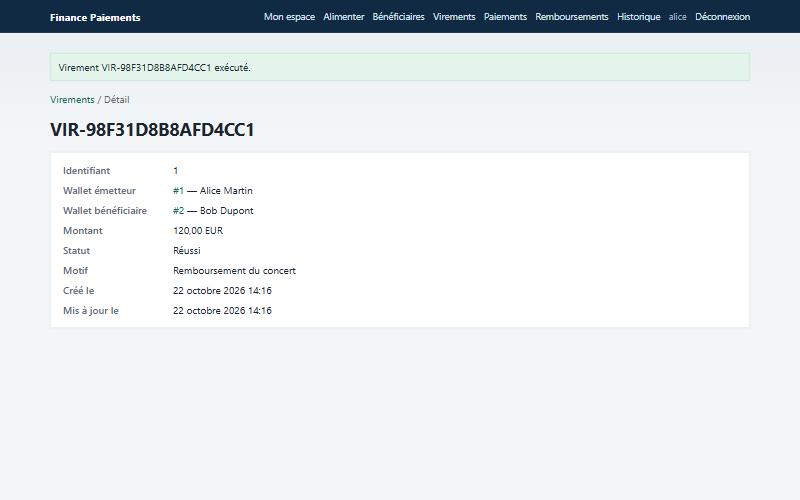
\includegraphics[width=\linewidth]{03-virement.jpg}\\[-0.2em]
  {\small (a) Virement exécuté}
\end{minipage}\hfill
\begin{minipage}{0.49\linewidth}\centering
  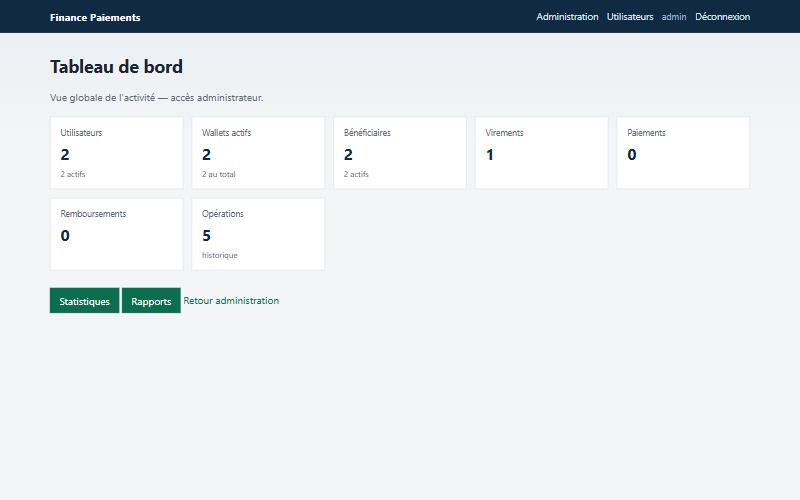
\includegraphics[width=\linewidth]{04-tableau-de-bord.jpg}\\[-0.2em]
  {\small (b) Tableau de bord administrateur}
\end{minipage}
\caption{Virement et pilotage}
\end{figure}

\begin{figure}[H]
\centering
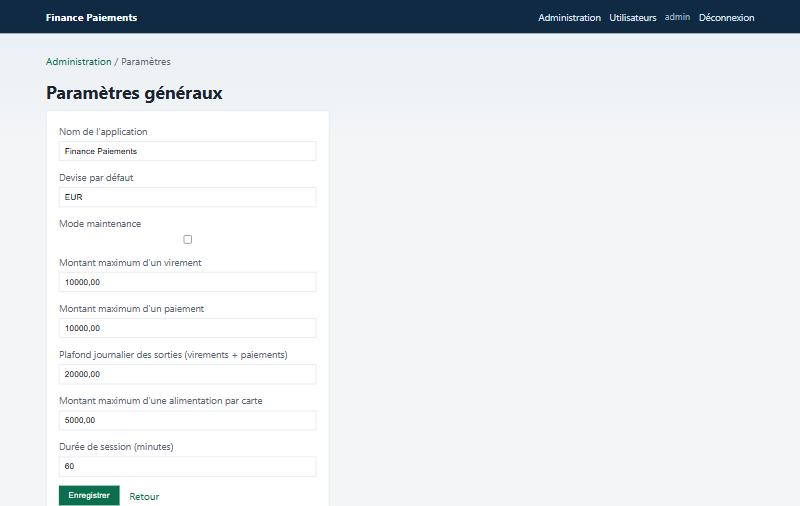
\includegraphics[width=0.62\linewidth]{05-parametres.jpg}
\caption{Paramètres : plafonds par opération, journalier et d'alimentation, maintenance}
\end{figure}

% =====================================================================
\chapter{Tests et validation}
% =====================================================================

\section{Stratégie}

\begin{table}[H]
\centering
\caption{Niveaux de test}
\begin{tabularx}{\linewidth}{@{}p{3.4cm}Y@{}}
\toprule
\entete \tete{Niveau} & \tete{Ce qui est vérifié} \\
\midrule
Unitaire & Règles métier isolées : solde, plafonds, montants, passerelle de carte. \\
Intégrité financière & Un échec en cours de transaction n'altère aucun solde. \\
Intégration & Requête HTTP complète : permissions, codes de retour, rendu des pages et de l'API. \\
Sécurité & Une attaque par test : accès aux données d'autrui, énumération, double soumission, force brute, CSRF. \\
Non-régression & Tout défaut corrigé reçoit un test. \\
\bottomrule
\end{tabularx}
\end{table}

\section{Résultats}

\begin{encadre}[title=Résultats de la campagne de tests (version \Version)]
\begin{tabularx}{\linewidth}{@{}YYYY@{}}
\textbf{\Large 169} tests & \textbf{\Large 169} réussis & \textbf{\Large 86\,\%} de couverture & \textbf{\Large 2} bases testées \\
\end{tabularx}
\end{encadre}

\begin{table}[H]
\centering
\caption{Répartition des tests par fichier}
\begin{tabularx}{\linewidth}{@{}p{5.2cm}C{1.2cm}C{1.3cm}Y@{}}
\toprule
\entete \tete{Fichier} & \tete{Tests} & \tete{Sprint} & \tete{Domaine} \\
\midrule
\code{test\_configuration.py} & 7 & 0 & Configuration \\
\code{test\_utilisateurs\_wallets.py} & 14 & 1 & Utilisateurs, portefeuilles \\
\code{test\_historique.py} & 11 & 2 & Historique \\
\code{test\_beneficiaires.py} & 12 & 3 & Bénéficiaires \\
\code{test\_virements.py} & 15 & 4 & Virements \\
\code{test\_paiements.py} & 13 & 5 & Paiements, remboursements \\
\code{test\_administration.py} & 8 & 6 & Administration \\
\code{test\_securite.py} & 12 & 7 & Security by Design \\
\code{test\_pilotage.py} & 11 & 8 & Pilotage \\
\code{test\_observabilite.py} & 9 & 9 & Observabilité \\
\code{test\_exports.py} & 9 & 10 & Exports \\
\code{test\_durcissement.py} & 48 & 11 & Audit de sécurité \\
\midrule
\textbf{Total} & \textbf{169} & & \\
\bottomrule
\end{tabularx}
\end{table}

\section{Matrice de traçabilité}
\label{sec:tracabilite}

\begin{longtable}{@{}p{3.8cm}p{10.2cm}@{}}
\caption{Matrice de traçabilité exigences / tests (extrait)}\\
\toprule
\entete \tete{Exigence} & \tete{Tests représentatifs} \\
\midrule
\endfirsthead
\toprule
\entete \tete{Exigence} & \tete{Tests représentatifs} \\
\midrule
\endhead
EF-01 Compte & \code{test\_inscription\_web\_cree\_compte\_wallet\_et\_session}\newline \code{test\_solde\_initial\_est\_zero} \\
EF-02 Connexion & \code{test\_client\_se\_connecte\_hors\_du\_site\_admin}\newline \code{test\_deconnexion\_post\_uniquement} \\
EF-04 Alimentation & \code{test\_alimentation\_acceptee\_credite\_et\_trace}\newline \code{test\_alimentation\_refusee\_ne\_credite\_pas} \\
EF-05 Historique & \code{test\_filtres\_type\_et\_statut}\newline \code{test\_historique\_automatique} \\
EF-06 Bénéficiaires & \code{test\_api\_ajout\_par\_email}\newline \code{test\_desactivation\_et\_reactivation} \\
EF-07 Virements & \code{test\_virement\_valide}\newline \code{test\_transaction\_atomique\_en\_cas\_echec\_historique} \\
EF-08 Paiements & \code{test\_paiement\_valide}\newline \code{test\_remboursement\_montant\_excessif} \\
EF-09 Idempotence & \code{test\_double\_soumission\_virement\_un\_seul\_debit}\newline \code{test\_api\_virement\_idempotency\_key} \\
EF-11 Plafonds & \code{test\_plafond\_virement}\newline \code{test\_plafond\_journalier\_cumule} \\
EF-12 Journal admin. & \code{test\_journal\_modification\_parametres\_et\_activation} \\
EF-13 Pilotage & \code{test\_dashboard\_compteurs}\newline \code{test\_statistiques\_filtre\_utilisateur} \\
EF-15 Exports & \code{test\_export\_tous\_types\_json}\newline \code{test\_export\_csv\_neutralise\_motif} \\
ENF-02 Cloisonnement & \code{test\_idor\_api\_utilisateurs\_wallets}\newline \code{test\_acces\_interdit\_autre\_proprietaire} \\
ENF-03 Annuaire & \code{test\_api\_refuse\_l\_ajout\_par\_identifiant}\newline \code{test\_formulaire\_beneficiaire\_ne\_liste\_pas\_les\_clients} \\
ENF-04 Force brute & \code{test\_blocage\_apres\_echecs}\newline \code{test\_blocage\_par\_adresse\_ip} \\
ENF-06 Carte & \code{test\_numero\_de\_carte\_jamais\_conserve} \\
ENF-08 Montants & \code{test\_montants\_invalides\_rejetes} \\
ENF-12 Production & \code{test\_production\_refuse\_de\_demarrer\_sans\_cle\_secrete} \\
\bottomrule
\end{longtable}

\section{Intégration continue}

\begin{figure}[H]
\centering
\begin{tikzpicture}[
  etape/.style={rectangle, rounded corners=3pt, draw=primaire, thick, fill=primaireclair,
                minimum height=1cm, text width=2.5cm, align=center, font=\scriptsize},
  fleche/.style={-{Stealth[length=2mm]}, thick, color=encre},
]
  \node[etape, fill=white, draw=gris] (push) at (0,0) {\textbf{push / PR}};
  \node[etape] (mig) at (3.2,0.8) {Migrations à jour\\{\tiny makemigrations --check}};
  \node[etape] (tst) at (6.4,0.8) {Tests + couverture\\{\tiny seuil 80\,\%}};
  \node[etape] (dep) at (9.6,0.8) {Configuration de production\\{\tiny check --deploy}};
  \node[etape] (pg) at (6.4,-0.8) {Suite complète sur PostgreSQL 16};
  \draw[fleche] (push) -- (mig.west);
  \draw[fleche] (mig) -- (tst);
  \draw[fleche] (tst) -- (dep);
  \draw[fleche] (push) |- (pg);
\end{tikzpicture}
\caption{Pipeline d'intégration continue (deux jobs parallèles)}
\end{figure}

% =====================================================================
\chapter{Audit de sécurité}
% =====================================================================

\section{Démarche}

Le prototype 3 a introduit la \emph{Security by Design} (cloisonnement, plafonds,
maintenance, journal d'administration). À la fin du prototype 4, l'auteur a audité
son propre code : lecture des services, des vues et des 31 routes d'API, puis
parcours manuel complet en tant que client et administrateur. Le constat le plus
instructif : deux défauts \emph{bloquants} n'étaient détectés par aucun test, car
les tests appelaient directement les services sans jouer le parcours réel d'un client.

\section{Modèle de menace}

\begin{table}[H]
\centering
\caption{Actifs, menaces et attaquants}
\begin{tabularx}{\linewidth}{@{}p{3.4cm}Yp{3.4cm}@{}}
\toprule
\entete \tete{Actif} & \tete{Menace} & \tete{Attaquant} \\
\midrule
Fonds des clients & Double débit, solde négatif, contournement des plafonds & Client, erreur réseau \\
Annuaire des clients & Collecte des noms et e-mails (hameçonnage ciblé) & Client authentifié \\
Comptes & Deviner un mot de passe, login CSRF & Attaquant externe \\
Données d'autrui & Lire un portefeuille ou un historique étranger & Client authentifié \\
Poste de l'administrateur & Formule exécutée à l'ouverture d'un export & Client malveillant \\
\bottomrule
\end{tabularx}
\end{table}

\section{Défauts identifiés et corrigés}

\begin{longtable}{@{}p{0.8cm}p{2.1cm}p{5.4cm}p{5.75cm}@{}}
\caption{Résultats de l'audit de sécurité (sprint 11)}\\
\toprule
\entete \tete{ID} & \tete{Gravité} & \tete{Défaut constaté} & \tete{Correction} \\
\midrule
\endfirsthead
\toprule
\entete \tete{ID} & \tete{Gravité} & \tete{Défaut constaté} & \tete{Correction} \\
\midrule
\endhead
F1 & \gravite{rouge}{Critique} & Annuaire énumérable : l'API renvoyait nom et e-mail d'un client à partir d'un identifiant séquentiel ; le formulaire web listait tous les clients. & Ajout de bénéficiaire par e-mail exact, message d'erreur générique. \\
F2 & \gravite{rouge}{Bloquant} & Aucun espace client : seule la connexion \code{/admin/}, réservée au personnel, existait. & Inscription, connexion, déconnexion (web et API), espace client. \\
F3 & \gravite{rouge}{Bloquant} & Aucun moyen d'approvisionner un portefeuille : l'application était inutilisable. & Alimentation par carte via une passerelle simulée côté serveur. \\
F4 & \gravite{orange}{Élevée} & Double débit sur double clic ou requête rejouée. & Clés d'idempotence et contrainte d'unicité en base. \\
F5 & \gravite{orange}{Élevée} & Plafond par opération contournable en plusieurs opérations. & Plafond journalier cumulé, contrôlé portefeuille verrouillé. \\
F6 & \gravite{jaune}{Moyenne} & Arrondi silencieux (\code{0.001} devenait \code{0.00}) ; erreur 500 sur \code{1e30}. & Validation stricte des montants. \\
F7 & \gravite{jaune}{Moyenne} & Injection de formules dans les exports CSV. & Neutralisation des cellules à risque. \\
F8 & \gravite{jaune}{Moyenne} & Force brute et login CSRF à l'ouverture de l'espace client. & Blocage temporaire, CSRF imposé, redirections sûres. \\
F9 & \gravite{jaune}{Moyenne} & Adresse IP falsifiable via \code{X-Forwarded-For}. & En-tête ignoré par défaut. \\
F10 & \gravite{jaune}{Moyenne} & Configuration non sûre par défaut. & Configuration de production dédiée, Docker non-root. \\
F11 & \gravite{bleu}{Qualité} & Fichiers en double interligne, nom de laboratoire visible. & Normalisation, renommage du produit. \\
\bottomrule
\end{longtable}

\section{Exemple détaillé : le double débit (F4)}

Sans protection, un double clic sur « Exécuter le virement » ou une requête renvoyée
après une coupure réseau produisait deux virements. La correction reprend le principe
des API de paiement réelles : chaque demande porte une \textbf{clé d'idempotence}, et
une clé déjà utilisée renvoie l'opération existante au lieu d'en créer une nouvelle.

\begin{lstlisting}[caption={Virement idempotent : vérification de la clé sous verrou}]
cle = parse_cle_idempotence(cle_idempotence)
if cle is not None:
    # Deux requêtes simultanées portant la même clé sont sérialisées :
    # la seconde retrouve le virement de la première.
    wallet_verrouille = Wallet.objects.select_for_update().filter(
        utilisateur=emetteur).first()
    existant = Virement.objects.filter(
        wallet_emetteur=wallet_verrouille, cle_idempotence=cle).first()
    if existant is not None:
        return existant, False          # aucun nouveau débit
\end{lstlisting}

\begin{lstlisting}[caption={Test : deux soumissions, un seul débit}]
def test_double_soumission_virement_un_seul_debit(utilisateur, lien_bob):
    premier = executer_virement(emetteur=utilisateur, beneficiaire_id=lien_bob.pk,
                                montant='100.00', cle_idempotence='cle-1')
    second = executer_virement(emetteur=utilisateur, beneficiaire_id=lien_bob.pk,
                               montant='100.00', cle_idempotence='cle-1')
    assert second.pk == premier.pk and second.est_rejeu is True
    assert utilisateur.wallet.solde == Decimal('900.00')   # un seul débit
\end{lstlisting}

% =====================================================================
\chapter{Déploiement}
% =====================================================================

\section{Environnements}

\begin{table}[H]
\centering
\caption{Configurations par environnement}
\begin{tabularx}{\linewidth}{@{}p{5.4cm}Y@{}}
\toprule
\entete \tete{Configuration} & \tete{Usage} \\
\midrule
\code{config.settings.local} & Démarrage rapide avec SQLite, sans Docker \\
\code{config.settings.development} & Développement avec PostgreSQL (Docker) \\
\code{config.settings.test} & Tests automatisés \\
\code{config.settings.test\_postgres} & Suite de tests sur PostgreSQL \\
\code{config.settings.production} & HTTPS, cookies sécurisés, HSTS, WhiteNoise, clé secrète obligatoire \\
\bottomrule
\end{tabularx}
\end{table}

\section{Mise en production}

Le fichier \code{docker-compose.prod.yml} démarre la base PostgreSQL (volume
persistant) et l'application : migrations, collecte des fichiers statiques, puis
Gunicorn exécuté par un utilisateur non privilégié. Le chiffrement TLS est assuré en
amont par un reverse proxy. Les plafonds, la devise, la durée de session et le mode
maintenance se règlent ensuite depuis l'administration.

\begin{lstlisting}[language=bash, caption={Lancement local en quelques commandes}, numbers=none]
pip install -r requirements-dev.txt
set DJANGO_SETTINGS_MODULE=config.settings.local
python backend/manage.py migrate
python backend/manage.py creer_comptes_demo
python backend/manage.py runserver 8001
\end{lstlisting}

% =====================================================================
\chapter{Maintenance et évolutions}
% =====================================================================

\section{Gestion de version}

Le dépôt Git utilise des messages de commit conventionnels et un versionnement
sémantique. Le fichier \code{CHANGELOG.md} retrace chaque version, de la
version 1.0.0 (prototypes 1 à 4) à la version \Version{} issue de l'audit.

\section{Limites connues}

\begin{itemize}
  \item La carte bancaire est simulée : la passerelle se remplace par un prestataire
  réel sans modifier le reste de l'application.
  \item Pas de double authentification : indispensable avant une mise en service réelle.
  \item Les compteurs de tentatives de connexion utilisent un cache mémoire, adapté à
  une instance unique.
\end{itemize}

\section{Évolutions envisagées}

\begin{itemize}
  \item Double authentification pour les opérations sensibles.
  \item Prestataire de paiement réel en mode test.
  \item Retrait vers un compte bancaire (SEPA).
  \item Test de bout en bout de chaque parcours client dans la suite automatisée.
\end{itemize}

% =====================================================================
\chapter{Conclusion}
% =====================================================================

Le projet a mené une plateforme de portefeuille électronique de l'expression des
besoins jusqu'à un déploiement de type production, en suivant toutes les phases du
cycle de vie du développement logiciel. Le \textbf{prototypage évolutif} a permis de
sécuriser très tôt le cœur sensible --- les mouvements de fonds --- puis de l'entourer,
prototype après prototype, d'administration, de pilotage et de traçabilité. La méthode
\textbf{Scrum} a structuré le travail en incréments testés et documentés.

\begin{encadre}[title=Bilan et rétrospective]
\textbf{Ce qui a bien fonctionné.} Le module unique de mouvements de fonds a rendu
simples l'ajout de l'idempotence et du plafond journalier ; les 121 tests existants ont
confirmé qu'aucune règle financière n'avait régressé.

\smallskip
\textbf{Ce que je ferais différemment.} Écrire dès le départ un test de bout en bout
par parcours utilisateur : il aurait révélé immédiatement qu'un client ne pouvait ni se
connecter ni approvisionner son portefeuille. Et planifier un audit de sécurité à la
fin de chaque prototype.
\end{encadre}

% =====================================================================
\appendix
\chapter{Annexes}
% =====================================================================

\section{Comptes et cartes de démonstration}

\begin{table}[H]
\centering
\caption{Comptes de démonstration (mode développement uniquement)}
\begin{tabular}{@{}llll@{}}
\toprule
\entete \tete{Rôle} & \tete{Identifiant} & \tete{Mot de passe} & \tete{Départ} \\
\midrule
Cliente & \code{alice} & \code{Alice-Demo-2026} & 1 500 EUR \\
Client & \code{bob} & \code{Bob-Demo-2026} & 300 EUR \\
Administrateur & \code{admin} & \code{Admin-Demo-2026} & --- \\
\bottomrule
\end{tabular}
\end{table}

\begin{table}[H]
\centering
\caption{Cartes de test de la passerelle simulée}
\begin{tabular}{@{}ll@{}}
\toprule
\entete \tete{Carte} & \tete{Résultat} \\
\midrule
\code{4242 4242 4242 4242} & Acceptée \\
\code{4000 0000 0000 0002} & Refusée (fonds insuffisants) \\
Numéro à clé de Luhn invalide & Rejeté, rien n'est enregistré \\
\bottomrule
\end{tabular}
\end{table}

\section{Organisation du dépôt}

\begin{table}[H]
\centering
\caption{Structure du dépôt}
\begin{tabularx}{\linewidth}{@{}p{5.7cm}Y@{}}
\toprule
\entete \tete{Dossier} & \tete{Contenu} \\
\midrule
\code{backend/} & Projet Django, configuration par environnement \\
\code{accounts/} \dots{} \code{observabilite/} & Modules métier (modèles, services, vues) \\
\code{api/} & API REST \\
\code{commun/} & Utilitaires transverses \\
\code{frontend/} & Gabarits HTML et CSS \\
\code{tests/} & 169 tests automatisés \\
\code{docker/} & Dockerfile, Compose de développement et de production \\
\code{docs/} & Documentation par phase du cycle de vie, ce rapport \\
\code{livrables/} & Rapports de sprint et audits \\
\bottomrule
\end{tabularx}
\end{table}

\end{document}
